%!TEX root = ../Bachelorseminar-RoboticSwarms.tex

	\begin{figure}[h]
		\label{venn_diagram}
		\caption{Super-awesome Venn-diagram}

		\centering

		\def\loclb{(180:2.0cm) circle (2.0cm)}
	  	\def\loclf{(0:2.0cm) circle (2.0cm)}
	  	\def\locrb{(90:2.0cm) circle (2.0cm)}
	  	\def\locrf{(270:2.0cm) circle (2.0cm)}

	    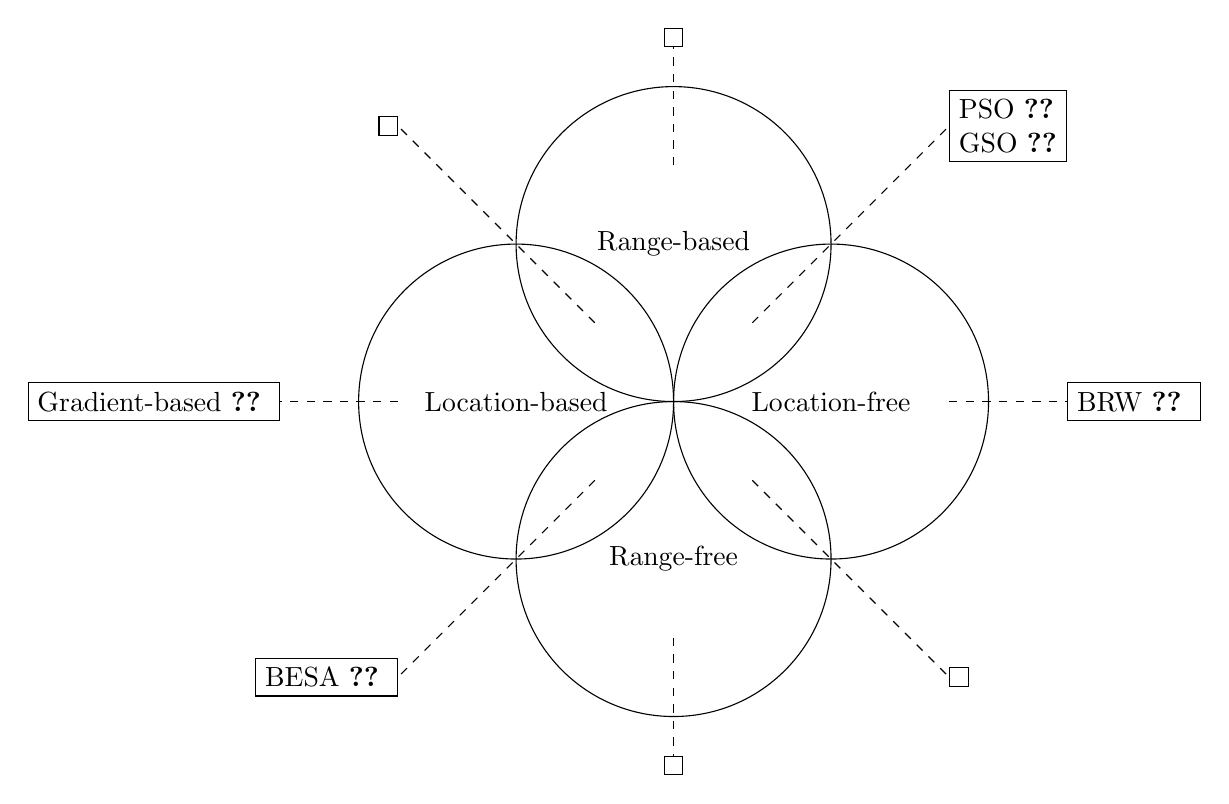
\begin{tikzpicture}
			% standard figures
			\draw \loclb node [text=black] {Location-based};
			\draw \loclf node [text=black] {Location-free};
			\draw \locrb node [text=black] {Range-based};
			\draw \locrf node [text=black] {Range-free};

			% Range-based location-free
			\draw[dashed,-] (1,1) -- (3.5,3.5) node[anchor=north west] {};
			\node[draw,align=left,anchor=west] at (3.5,3.5) {
				PSO \ref{sec:Localization}\\
				GSO \ref{sec:Localization}
			};

			% Range-free, location-free
			\draw[dashed,-] (1,-1) -- (3.5,-3.5) node[anchor=north west] {};
			\node[draw,align=left,anchor=west] at (3.5,-3.5) {

			};

			% location-free
			\draw[dashed,-] (3.5,0) -- (5,0) node[anchor=north west] {};
			\node[draw,align=left,anchor=west] at (5,0) {
				BRW \ref{sec:Localization}
			};

			% location-based
			\draw[dashed,-] (-3.5,0) -- (-5,0) node[anchor=north west] {};
			\node[draw,align=left,anchor=east] at (-5,0) {
				Gradient-based \ref{sec:Localization}
			};

			% Range-free, location-based
			\draw[dashed,-] (-1,-1) -- (-3.5,-3.5) node[anchor=north west] {};
			\node[draw,align=left,anchor=east] at (-3.5,-3.5) {
				BESA \ref{sec:Localization}
			};

			% Range-based, location-based
			\draw[dashed,-] (-1,1) -- (-3.5,3.5) node[anchor=north west] {};
			\node[draw,align=left,anchor=east] at (-3.5,3.5) {

			};

			% Range-based
			\draw[dashed,-] (0,3) -- (0,4.5) node[anchor=north west] {};
			\node[draw,align=left,anchor=south] at (0,4.5) {

			};

			% Range-free
			\draw[dashed,-] (0,-3) -- (0,-4.5) node[anchor=north west] {};
			\node[draw,align=left,anchor=north] at (0,-4.5) {
			
			};
		\end{tikzpicture}
    \end{figure}